\documentclass[border=10pt]{standalone}
\usepackage{pgfplots}
\pgfplotsset{compat=1.18}
\begin{document}
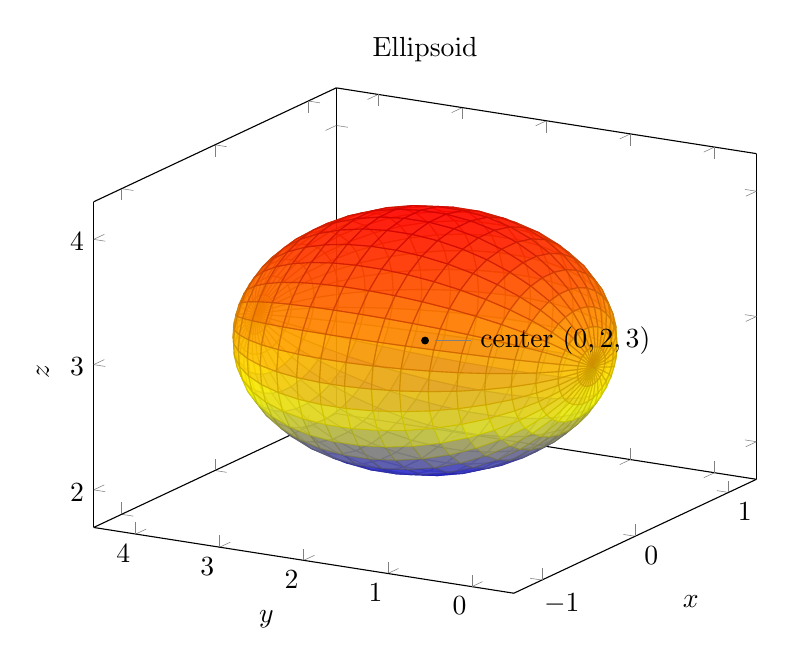
\begin{tikzpicture}
\begin{axis}[
  width=10cm, height=8cm,
  view={-60}{22},
  xlabel={$x$}, ylabel={$y$}, zlabel={$z$},
  xmin=-1.3, xmax=1.3, ymin=-0.5, ymax=4.5, zmin=1.7, zmax=4.3,
  grid=none,
  title={Ellipsoid}
]
\addplot3[
  surf,
  opacity=0.75,
  domain=0:2*pi,
  y domain=0:pi,
  samples=35,
  samples y=22
]
({cos(deg(x))*sin(deg(y))},
 {2+2*cos(deg(y))},
 {3+sin(deg(x))*sin(deg(y))});
\addplot3[only marks, mark=*, mark size=1.2pt, black] coordinates {(0,2,3)};
\node[pin=right:{center $(0,2,3)$}] at (axis cs:0,2,3) {};
\end{axis}
\end{tikzpicture}
\end{document}